\chapter{Marseilles-The Arrival}

On the 24th of February, 1815, the look-out at Notre-Dame de la Garde
signalled the three-master, the \textit{Pharaon} from Smyrna, Trieste, and
Naples.

As usual, a pilot put off immediately, and rounding the Château d’If,
got on board the vessel between Cape Morgiou and Rion island.

Immediately, and according to custom, the ramparts of Fort Saint-Jean
were covered with spectators; it is always an event at Marseilles for a
ship to come into port, especially when this ship, like the \textit{Pharaon},
has been built, rigged, and laden at the old Phocee docks, and belongs
to an owner of the city.

The ship drew on and had safely passed the strait, which some volcanic
shock has made between the Calasareigne and Jaros islands; had doubled
Pomègue, and approached the harbor under topsails, jib, and spanker,
but so slowly and sedately that the idlers, with that instinct which is
the forerunner of evil, asked one another what misfortune could have
happened on board. However, those experienced in navigation saw plainly
that if any accident had occurred, it was not to the vessel herself,
for she bore down with all the evidence of being skilfully handled, the
anchor a-cockbill, the jib-boom guys already eased off, and standing by
the side of the pilot, who was steering the \textit{Pharaon} towards the
narrow entrance of the inner port, was a young man, who, with activity
and vigilant eye, watched every motion of the ship, and repeated each
direction of the pilot.

The vague disquietude which prevailed among the spectators had so much
affected one of the crowd that he did not await the arrival of the
vessel in harbor, but jumping into a small skiff, desired to be pulled
alongside the \textit{Pharaon}, which he reached as she rounded into La
Réserve basin.

When the young man on board saw this person approach, he left his
station by the pilot, and, hat in hand, leaned over the ship’s
bulwarks.

He was a fine, tall, slim young fellow of eighteen or twenty, with
black eyes, and hair as dark as a raven’s wing; and his whole
appearance bespoke that calmness and resolution peculiar to men
accustomed from their cradle to contend with danger.

“Ah, is it you, Dantès?” cried the man in the skiff. “What’s the
matter? and why have you such an air of sadness aboard?”

“A great misfortune, M. Morrel,” replied the young man, “a great
misfortune, for me especially! Off Civita Vecchia we lost our brave
Captain Leclere.”

“And the cargo?” inquired the owner, eagerly.

“Is all safe, M. Morrel; and I think you will be satisfied on that
head. But poor Captain Leclere——”

“What happened to him?” asked the owner, with an air of considerable
resignation. “What happened to the worthy captain?”

“He died.”

“Fell into the sea?”

“No, sir, he died of brain-fever in dreadful agony.” Then turning to
the crew, he said, “Bear a hand there, to take in sail!”

All hands obeyed, and at once the eight or ten seamen who composed the
crew, sprang to their respective stations at the spanker brails and
outhaul, topsail sheets and halyards, the jib downhaul, and the topsail
clewlines and buntlines. The young sailor gave a look to see that his
orders were promptly and accurately obeyed, and then turned again to
the owner.

“And how did this misfortune occur?” inquired the latter, resuming the
interrupted conversation.

\begin{figure}[h]
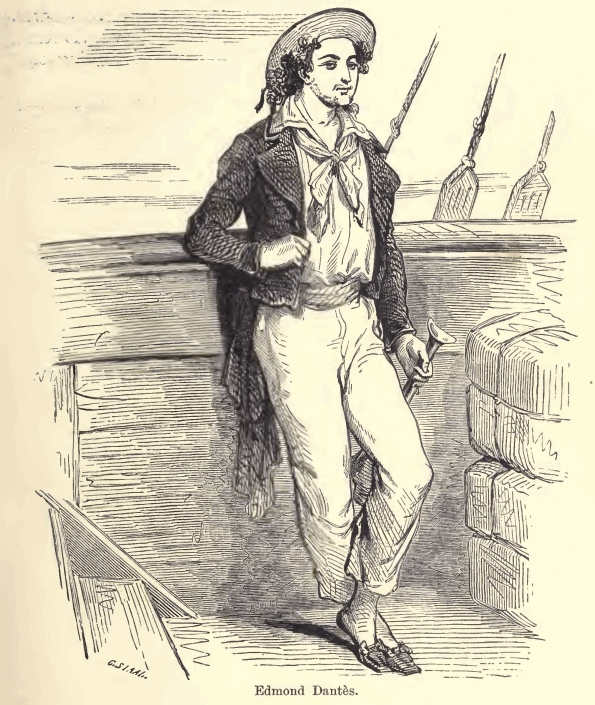
\includegraphics[width=\textwidth]{0023m.jpg}
\end{figure}

“Alas, sir, in the most unexpected manner. After a long talk with the
harbor-master, Captain Leclere left Naples greatly disturbed in mind.
In twenty-four hours he was attacked by a fever, and died three days
afterwards. We performed the usual burial service, and he is at his
rest, sewn up in his hammock with a thirty-six-pound shot at his head
and his heels, off El Giglio island. We bring to his widow his sword
and cross of honor. It was worth while, truly,” added the young man
with a melancholy smile, “to make war against the English for ten
years, and to die in his bed at last, like everybody else.”

“Why, you see, Edmond,” replied the owner, who appeared more comforted
at every moment, “we are all mortal, and the old must make way for the
young. If not, why, there would be no promotion; and since you assure
me that the cargo——”

“Is all safe and sound, M. Morrel, take my word for it; and I advise
you not to take 25,000 francs for the profits of the voyage.”

Then, as they were just passing the Round Tower, the young man shouted:
“Stand by there to lower the topsails and jib; brail up the spanker!”

The order was executed as promptly as it would have been on board a
man-of-war.

“Let go—and clue up!” At this last command all the sails were lowered,
and the vessel moved almost imperceptibly onwards.

“Now, if you will come on board, M. Morrel,” said Dantès, observing the
owner’s impatience, “here is your supercargo, M. Danglars, coming out
of his cabin, who will furnish you with every particular. As for me, I
must look after the anchoring, and dress the ship in mourning.”

The owner did not wait for a second invitation. He seized a rope which
Dantès flung to him, and with an activity that would have done credit
to a sailor, climbed up the side of the ship, while the young man,
going to his task, left the conversation to Danglars, who now came
towards the owner. He was a man of twenty-five or twenty-six years of
age, of unprepossessing countenance, obsequious to his superiors,
insolent to his subordinates; and this, in addition to his position as
responsible agent on board, which is always obnoxious to the sailors,
made him as much disliked by the crew as Edmond Dantès was beloved by
them.

“Well, M. Morrel,” said Danglars, “you have heard of the misfortune
that has befallen us?”

“Yes—yes: poor Captain Leclere! He was a brave and an honest man.”

“And a first-rate seaman, one who had seen long and honorable service,
as became a man charged with the interests of a house so important as
that of Morrel \& Son,” replied Danglars.

“But,” replied the owner, glancing after Dantès, who was watching the
anchoring of his vessel, “it seems to me that a sailor needs not be so
old as you say, Danglars, to understand his business, for our friend
Edmond seems to understand it thoroughly, and not to require
instruction from anyone.”

“Yes,” said Danglars, darting at Edmond a look gleaming with hate.
“Yes, he is young, and youth is invariably self-confident. Scarcely was
the captain’s breath out of his body when he assumed the command
without consulting anyone, and he caused us to lose a day and a half at
the Island of Elba, instead of making for Marseilles direct.”

\begin{figure}[h]
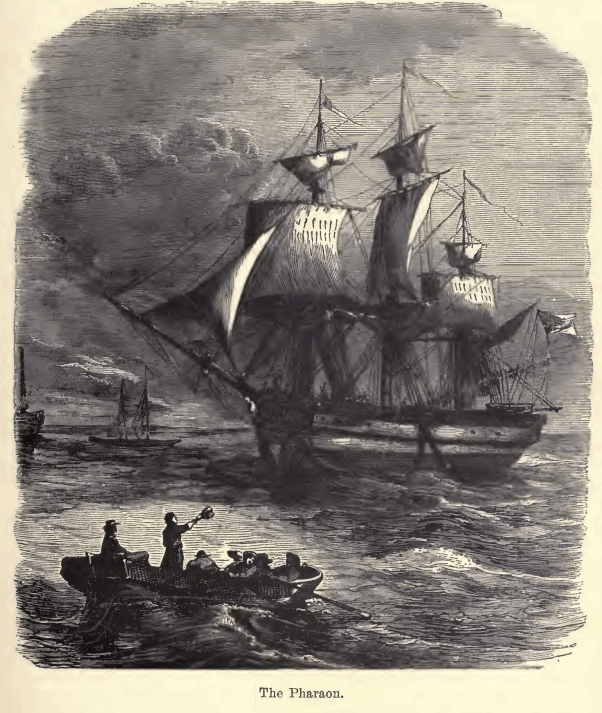
\includegraphics[width=\textwidth]{0025m.jpg}
\end{figure}

“As to taking command of the vessel,” replied Morrel, “that was his
duty as captain’s mate; as to losing a day and a half off the Island of
Elba, he was wrong, unless the vessel needed repairs.”

“The vessel was in as good condition as I am, and as, I hope you are,
M. Morrel, and this day and a half was lost from pure whim, for the
pleasure of going ashore, and nothing else.”

“Dantès,” said the shipowner, turning towards the young man, “come this
way!”

“In a moment, sir,” answered Dantès, “and I’m with you.” Then calling
to the crew, he said, “Let go!”

The anchor was instantly dropped, and the chain ran rattling through
the port-hole. Dantès continued at his post in spite of the presence of
the pilot, until this manœuvre was completed, and then he added,
“Half-mast the colors, and square the yards!”

“You see,” said Danglars, “he fancies himself captain already, upon my
word.”

“And so, in fact, he is,” said the owner.

“Except your signature and your partner’s, M. Morrel.”

“And why should he not have this?” asked the owner; “he is young, it is
true, but he seems to me a thorough seaman, and of full experience.”

A cloud passed over Danglars’ brow.

“Your pardon, M. Morrel,” said Dantès, approaching, “the vessel now
rides at anchor, and I am at your service. You hailed me, I think?”

Danglars retreated a step or two. “I wished to inquire why you stopped
at the Island of Elba?”

“I do not know, sir; it was to fulfil the last instructions of Captain
Leclere, who, when dying, gave me a packet for Marshal Bertrand.”

“Then did you see him, Edmond?”

“Who?”

“The marshal.”

“Yes.”

Morrel looked around him, and then, drawing Dantès on one side, he said
suddenly—

“And how is the emperor?”

“Very well, as far as I could judge from the sight of him.”

“You saw the emperor, then?”

“He entered the marshal’s apartment while I was there.”

“And you spoke to him?”

“Why, it was he who spoke to me, sir,” said Dantès, with a smile.

“And what did he say to you?”

“Asked me questions about the vessel, the time she left Marseilles, the
course she had taken, and what was her cargo. I believe, if she had not
been laden, and I had been her master, he would have bought her. But I
told him I was only mate, and that she belonged to the firm of Morrel \&
Son. ‘Ah, yes,’ he said, ‘I know them. The Morrels have been shipowners
from father to son; and there was a Morrel who served in the same
regiment with me when I was in garrison at Valence.’”

“\textit{Pardieu!} and that is true!” cried the owner, greatly delighted. “And
that was Policar Morrel, my uncle, who was afterwards a captain.
Dantès, you must tell my uncle that the emperor remembered him, and you
will see it will bring tears into the old soldier’s eyes. Come, come,”
continued he, patting Edmond’s shoulder kindly, “you did very right,
Dantès, to follow Captain Leclere’s instructions, and touch at Elba,
although if it were known that you had conveyed a packet to the
marshal, and had conversed with the emperor, it might bring you into
trouble.”

\begin{figure}[h]
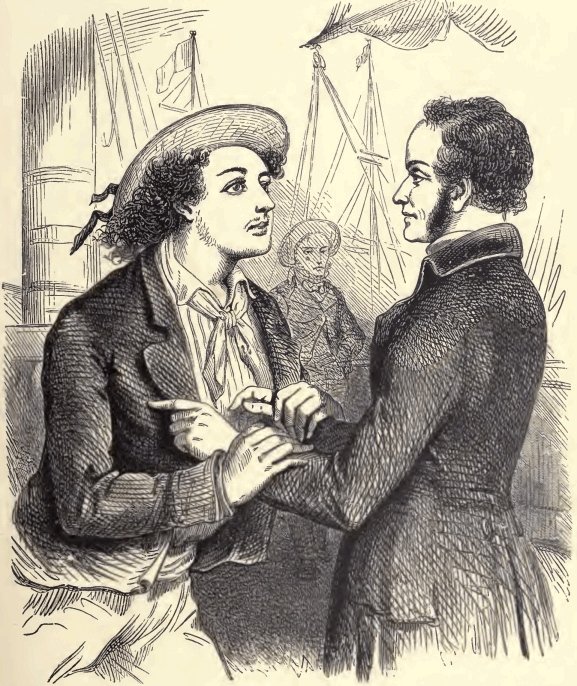
\includegraphics[width=\textwidth]{0027m.jpg}
\end{figure}

“How could that bring me into trouble, sir?” asked Dantès; “for I did
not even know of what I was the bearer; and the emperor merely made
such inquiries as he would of the first comer. But, pardon me, here are
the health officers and the customs inspectors coming alongside.” And
the young man went to the gangway. As he departed, Danglars approached,
and said,—

“Well, it appears that he has given you satisfactory reasons for his
landing at Porto-Ferrajo?”

“Yes, most satisfactory, my dear Danglars.”

“Well, so much the better,” said the supercargo; “for it is not
pleasant to think that a comrade has not done his duty.”

“Dantès has done his,” replied the owner, “and that is not saying much.
It was Captain Leclere who gave orders for this delay.”

“Talking of Captain Leclere, has not Dantès given you a letter from
him?”

“To me?—no—was there one?”

“I believe that, besides the packet, Captain Leclere confided a letter
to his care.”

“Of what packet are you speaking, Danglars?”

“Why, that which Dantès left at Porto-Ferrajo.”

“How do you know he had a packet to leave at Porto-Ferrajo?”

Danglars turned very red.

“I was passing close to the door of the captain’s cabin, which was half
open, and I saw him give the packet and letter to Dantès.”

“He did not speak to me of it,” replied the shipowner; “but if there be
any letter he will give it to me.”

Danglars reflected for a moment. “Then, M. Morrel, I beg of you,” said
he, “not to say a word to Dantès on the subject. I may have been
mistaken.”

At this moment the young man returned; Danglars withdrew.

“Well, my dear Dantès, are you now free?” inquired the owner.

“Yes, sir.”

“You have not been long detained.”

“No. I gave the custom-house officers a copy of our bill of lading; and
as to the other papers, they sent a man off with the pilot, to whom I
gave them.”

“Then you have nothing more to do here?”

“No—everything is all right now.”

“Then you can come and dine with me?”

“I really must ask you to excuse me, M. Morrel. My first visit is due
to my father, though I am not the less grateful for the honor you have
done me.”

\begin{figure}[h]
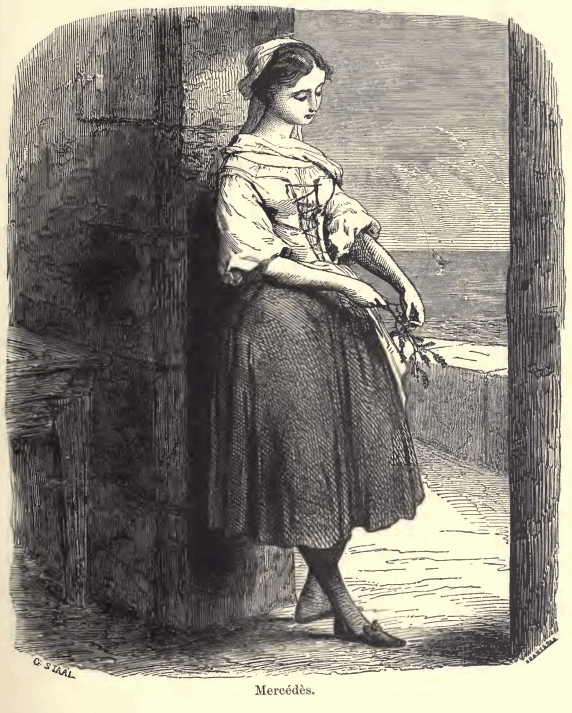
\includegraphics[width=\textwidth]{0029m.jpg}
\end{figure}

“Right, Dantès, quite right. I always knew you were a good son.”

“And,” inquired Dantès, with some hesitation, “do you know how my
father is?”

“Well, I believe, my dear Edmond, though I have not seen him lately.”

“Yes, he likes to keep himself shut up in his little room.”

“That proves, at least, that he has wanted for nothing during your
absence.”

Dantès smiled. “My father is proud, sir, and if he had not a meal left,
I doubt if he would have asked anything from anyone, except from
Heaven.”

“Well, then, after this first visit has been made we shall count on
you.”

“I must again excuse myself, M. Morrel, for after this first visit has
been paid I have another which I am most anxious to pay.”

“True, Dantès, I forgot that there was at the Catalans someone who
expects you no less impatiently than your father—the lovely Mercédès.”

Dantès blushed.

“Ah, ha,” said the shipowner, “I am not in the least surprised, for she
has been to me three times, inquiring if there were any news of the
\textit{Pharaon}. \textit{Peste!} Edmond, you have a very handsome mistress!”

“She is not my mistress,” replied the young sailor, gravely; “she is my
betrothed.”

“Sometimes one and the same thing,” said Morrel, with a smile.

“Not with us, sir,” replied Dantès.

“Well, well, my dear Edmond,” continued the owner, “don’t let me detain
you. You have managed my affairs so well that I ought to allow you all
the time you require for your own. Do you want any money?”

“No, sir; I have all my pay to take—nearly three months’ wages.”

“You are a careful fellow, Edmond.”

“Say I have a poor father, sir.”

“Yes, yes, I know how good a son you are, so now hasten away to see
your father. I have a son too, and I should be very wroth with those
who detained him from me after a three months’ voyage.”

“Then I have your leave, sir?”

“Yes, if you have nothing more to say to me.”

“Nothing.”

“Captain Leclere did not, before he died, give you a letter for me?”

“He was unable to write, sir. But that reminds me that I must ask your
leave of absence for some days.”

“To get married?”

“Yes, first, and then to go to Paris.”

“Very good; have what time you require, Dantès. It will take quite six
weeks to unload the cargo, and we cannot get you ready for sea until
three months after that; only be back again in three months, for the
\textit{Pharaon},” added the owner, patting the young sailor on the back,
“cannot sail without her captain.”

“Without her captain!” cried Dantès, his eyes sparkling with animation;
“pray mind what you say, for you are touching on the most secret wishes
of my heart. Is it really your intention to make me captain of the
\textit{Pharaon}?”

“If I were sole owner we’d shake hands on it now, my dear Dantès, and
call it settled; but I have a partner, and you know the Italian
proverb—\textit{Chi ha compagno ha padrone}—‘He who has a partner has a
master.’ But the thing is at least half done, as you have one out of
two votes. Rely on me to procure you the other; I will do my best.”

“Ah, M. Morrel,” exclaimed the young seaman, with tears in his eyes,
and grasping the owner’s hand, “M. Morrel, I thank you in the name of
my father and of Mercédès.”

“That’s all right, Edmond. There’s a providence that watches over the
deserving. Go to your father; go and see Mercédès, and afterwards come
to me.”

“Shall I row you ashore?”

“No, thank you; I shall remain and look over the accounts with
Danglars. Have you been satisfied with him this voyage?”

“That is according to the sense you attach to the question, sir. Do you
mean is he a good comrade? No, for I think he never liked me since the
day when I was silly enough, after a little quarrel we had, to propose
to him to stop for ten minutes at the island of Monte Cristo to settle
the dispute—a proposition which I was wrong to suggest, and he quite
right to refuse. If you mean as responsible agent when you ask me the
question, I believe there is nothing to say against him, and that you
will be content with the way in which he has performed his duty.”

“But tell me, Dantès, if you had command of the \textit{Pharaon} should you be
glad to see Danglars remain?”

“Captain or mate, M. Morrel, I shall always have the greatest respect
for those who possess the owners’ confidence.”

“That’s right, that’s right, Dantès! I see you are a thoroughly good
fellow, and will detain you no longer. Go, for I see how impatient you
are.”

“Then I have leave?”

“Go, I tell you.”

“May I have the use of your skiff?”

“Certainly.”

“Then, for the present, M. Morrel, farewell, and a thousand thanks!”

“I hope soon to see you again, my dear Edmond. Good luck to you.”

The young sailor jumped into the skiff, and sat down in the stern
sheets, with the order that he be put ashore at La Canebière. The two
oarsmen bent to their work, and the little boat glided away as rapidly
as possible in the midst of the thousand vessels which choke up the
narrow way which leads between the two rows of ships from the mouth of
the harbor to the Quai d’Orléans.

The shipowner, smiling, followed him with his eyes until he saw him
spring out on the quay and disappear in the midst of the throng, which
from five o’clock in the morning until nine o’clock at night, swarms in
the famous street of La Canebière,—a street of which the modern
Phocéens are so proud that they say with all the gravity in the world,
and with that accent which gives so much character to what is said, “If
Paris had La Canebière, Paris would be a second Marseilles.” On turning
round the owner saw Danglars behind him, apparently awaiting orders,
but in reality also watching the young sailor,—but there was a great
difference in the expression of the two men who thus followed the
movements of Edmond Dantès.
